\newpage
\section{Hotspot Analysis}
Heat conduction (or heat diffusion) is the process by which thermal energy spreads within a material due to temperature differences. In two dimensions, this phenomenon can be represented as heat spreading across a plate or surface over time. Numerical simulations of heat conduction are widely used in engineering, physics, and high-performance computing to predict temperature distribution and analyze thermal effects.

\begin{center}
    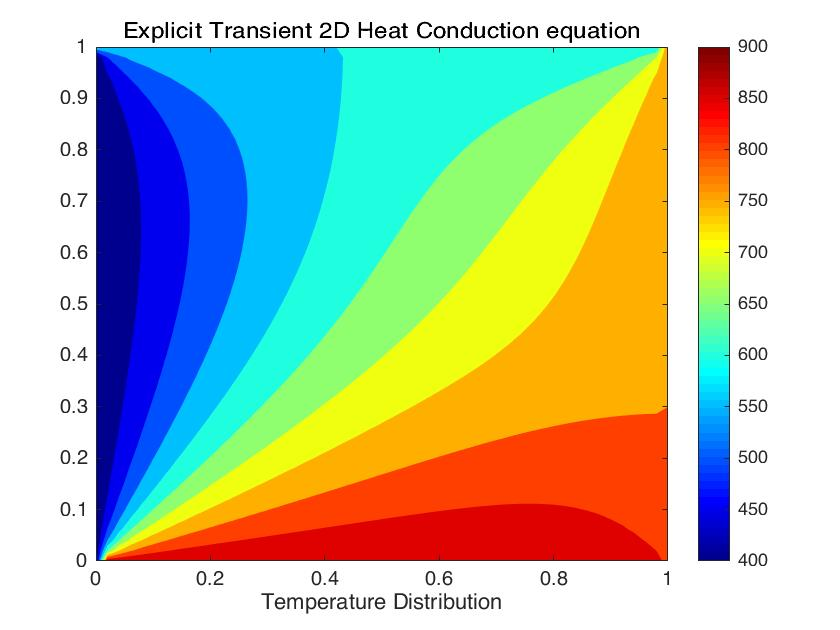
\includegraphics[width=0.6\textwidth]{assets/hotspots/heat_diffusion_simulation.jpg}
    \captionof{figure}{Illustration of 2D heat conduction simulation.}
\end{center}

\noindent
The formula to represent 2D heat conduction is given as follows:
\[
\frac{\partial T}{\partial t} = \alpha \left( \frac{\partial^2 T}{\partial x^2} + \frac{\partial^2 T}{\partial y^2} \right)
\]

where:
\begin{itemize}
    \item $T$ is temperature;
    \item $t$ is time;
    \item $\alpha$ is the thermal diffusivity;
    \item $(x,y)$ are points in a grid.
\end{itemize}

\noindent
To solve this problem numerically, one possible finite difference approximation is:

\[
\frac{\Delta T}{\Delta t} =
\frac{T_{i,j}^{n+1} - T_{i,j}^n}{\Delta t} = \alpha \left( 
\frac{T_{i+1,j}^n - 2T_{i,j}^n + T_{i-1,j}^n}{(\Delta x)^2} + 
\frac{T_{i,j+1}^n - 2T_{i,j}^n + T_{i,j-1}^n}{(\Delta y)^2} 
\right)
\]

where:
\begin{itemize}
    \item $\Delta t$ is the timestep;
    \item $i,j$ are indices in the grid;
    \item $n$ indicates the current timestep, so $T_{i,j}^n$ is the temperature at point $(i,j)$ at time $t=n \Delta t$, and $T_{i,j}^{n+1}$ is the temperature at the next timestep $t=(n+1) \Delta t$.
\end{itemize}

\noindent
In the beginning, the boundary points of the grid are assigned with initial temperatures, while the inner points update their temperature iteratively according to the formula above.\\

\noindent
TODO: aggiungere una fonte di calore concentrica al centro della griglia.

